\documentclass[conference,compsoc]{IEEEtran}
\usepackage{cite}
\usepackage{amsmath,amssymb,amsfonts}
\usepackage{graphicx}
\usepackage{textcomp}
\usepackage{xcolor}
\PassOptionsToPackage{hyphens}{url}
\usepackage[hidelinks]{hyperref}
\usepackage{algorithm}
\usepackage{algpseudocode}
\usepackage{tikz}
\usetikzlibrary{shapes.geometric, arrows.meta, positioning, fit, backgrounds, calc}
\usepackage{booktabs}
\usepackage{tabularx}
\usepackage{array}
\usepackage{multirow}
\usepackage{comment}
\newcommand{\linebreakand}{%
  \end{@IEEEauthorhalign}
  \hfill\mbox{}\par
  \mbox{}\hfill\begin{@IEEEauthorhalign}
}

\newcommand{\tightlist}{}
\newcolumntype{Y}{>{\raggedright\arraybackslash}X}

\begin{document}

\title{Graph-Augmented Hybrid RAG for CVE-to-CWE Mapping with Compact Open Large Language Models}

\author{}

\maketitle

\begin{abstract}
Mapping Common Vulnerabilities and Exposures (CVE) records to root-cause Common Weakness Enumeration (CWE) categories supports vulnerability triage, remediation planning, and security analytics. State-of-the-art results on this task have so far come from proprietary frontier models, models with extensive cybersecurity continued pre-training, or task-specific fine-tuned classifiers---each of which constrains reproducibility, local deployment, or methodological clarity. We present a Graph-Augmented Hybrid RAG system that pairs a single compact off-the-shelf open-source language model---with no cybersecurity-domain training and no task-specific fine-tuning---with a multi-stage retrieval pipeline over two public knowledge sources: the NIST National Vulnerability Database and the official CWE corpus. The pipeline combines BM25 and dense hybrid retrieval, structured CVE-to-CWE bridge injection from NVD weakness fields, weighted nearest-neighbor CWE voting over the mapped corpus, and BGE-Reranker-Base cross-encoder reranking. On CTI-Bench RCM, the system reaches 90.9\% strict accuracy and simultaneously surpasses every leading reference point on this task: GPT-4 (72.0\%, the published no-retrieval frontier anchor) by 18.9 percentage points, Cisco's cybersecurity-continued-pretrained Foundation-Sec-8B-R (75.3\%) by 15.6 percentage points, the strongest published open-source task-specific fine-tuned classifier (75.6\%) by 15.3 percentage points, and Google's closed cybersecurity-specialized Sec-Gemini v1 ($\sim$86\%). This headline decomposes into 92.7\% on the 903 NVD-mapped CVEs and 74.2\% on the 97 NVD-unmapped CVEs where no structured CWE lookup is available. The shipped primary model uses less than half the parameter count of every other open-source baseline on the leaderboard, and the full system runs locally on consumer GPUs. To establish that the result is carried by the retrieval pipeline rather than any LLM-side cybersecurity capability, we measure zero-shot vs.\ with-RAG accuracy for four open-source compact models spanning entirely different post-training regimes---reasoning distillation, RAG-tuned instruction following, and thinking-enabled instruction following---none with cybersecurity continued pre-training or task-specific fine-tuning. Their zero-shot accuracy spans 17.9\% to 69.6\%; under the same retrieval pipeline and the same benchmark-clean prompt they all converge to 82.1\% to 90.9\%, with RAG contributing between +20.7 and +73.0 percentage points per model. Every paired-with-RAG configuration exceeds GPT-4 by at least 10.0 percentage points and the strongest open-source fine-tuned specialist by at least 6.4 percentage points. The retrieval pipeline---not LLM cybersecurity specialization, reasoning post-training, or task fine-tuning---is the load-bearing component of the system.
\end{abstract}

\begin{IEEEkeywords}
cyber threat intelligence, CVE, CWE, retrieval-augmented generation, hybrid retrieval, vulnerability classification, root-cause mapping
\end{IEEEkeywords}

\section{Introduction}

Mapping newly disclosed Common Vulnerabilities and Exposures (CVE) records to root-cause Common Weakness Enumeration (CWE) identifiers is a recurring task in cyber threat intelligence (CTI). The mapping determines how analysts group vulnerabilities, select mitigations, prioritize remediation, and connect newly disclosed flaws to existing weakness taxonomies. Errors in this step propagate into downstream analysis, so CVE-to-CWE mapping is a narrow but important target for automation.

Large proprietary language models can perform this mapping when given only the CVE description, but their use introduces deployment costs: paid API access, transmission of vulnerability data to a third party, and limited reproducibility. Security-specialized open models have narrowed the gap, reaching up to 75.6\% on the CTI-Bench RCM benchmark \cite{mosievskiy-2026}, yet still fall short of closed security systems reporting around 85--86\% \cite{google-2025a,google-2025b}. For reference, GPT-4, the published no-retrieval frontier anchor for this benchmark, scores 72.0\% \cite{alam-2024}. Local open-source compact models without retrieval augmentation span a wide band on the same benchmark, from 44.7\% for LLaMA3-8B \cite{alam-2024} up to 75.3\% for the cybersecurity-continued-pretrained Foundation-Sec-8B-R \cite{yang-2026}.

This paper studies whether local compact general-purpose open-source language models, with no cybersecurity continued pre-training and no task-specific fine-tuning, can close that gap by reading public vulnerability knowledge at inference time. We build a graph-augmented hybrid retrieval-augmented generation (RAG) pipeline over two public sources: the National Vulnerability Database (NVD) CVE corpus \cite{national-2024} and the official MITRE CWE corpus \cite{mitre-2024a}. The pipeline combines BM25 and dense retrieval, explicit CVE-to-CWE bridge injection from structured NVD weakness fields, weighted nearest-neighbor voting over the mapped CVE corpus, and cross-encoder reranking. A single 3.8B-parameter open-source general-purpose model, Phi-4-mini-reasoning, serves as the primary final-answer model on every CTI-Bench query, whether the CVE has a structured NVD CWE assignment or not. We evaluate the same retrieval pipeline with three additional primary models spanning distinct post-training regimes to verify that the result is carried by retrieval rather than by any one LLM's capability.

The central research question is: under the CTI-Bench single-answer protocol, how far can local open-source compact general-purpose models go when paired with a retrieval pipeline over public CVE and CWE data, without any domain-specific continued pre-training or task-specific fine-tuning of the final-answer model?

Our contributions are as follows.
\begin{itemize}
\item We present a two-source graph-augmented hybrid RAG architecture for CVE-to-CWE root-cause mapping using only public NVD and CWE data.
\item We empirically compare four open-source compact (3.8B--8B) candidate primary models under the same retrieval pipeline, spanning distinct post-training regimes (two reasoning distillations, one RAG-tuned instruct, one thinking-enabled instruct), and select Phi-4-mini-reasoning (3.8B), the strongest candidate with neither cybersecurity continued pre-training nor task-specific fine-tuning, as the shipped primary.
\item We evaluate the full pipeline on all 1{,}000 CTI-Bench RCM queries and report 90.9\% strict accuracy, surpassing the strongest published open-source generative baseline by 15.3 percentage points and exceeding GPT-4, the published no-retrieval anchor, by 18.9 percentage points, using less than half the parameter count of every other open-source LLM baseline on the leaderboard.
\item We demonstrate the model-independence of the result. Under the same benchmark-clean context-only prompt, replacing the primary with IBM Granite 4.1-8B, a general-purpose RAG-tuned instruct model with no cybersecurity training, no reasoning post-training, and no task-specific fine-tuning, still reaches 85.6\% with our pipeline, up from 63.6\% zero-shot: a +22.0 percentage-point lift attributable purely to retrieval. Even this no-cybersecurity-knowledge variant exceeds the strongest published open-source fine-tuned specialist by 10.0 percentage points and GPT-4 by 13.6 percentage points, isolating retrieval as the load-bearing component of the system.
\end{itemize}

\section{Background and Related Work}

Prior work on automated CVE-to-CWE classification and RAG-based security analytics falls into three lines: general retrieval and reranking foundations, CVE-to-CWE classification methods, and security-tuned LLMs. We review each in turn.

\subsection{Retrieval-Augmented Generation}

Retrieval-Augmented Generation (RAG) combines a parametric generator with non-parametric retrieval over an external corpus \cite{lewis-2020}. This decoupling is central to our design: instead of fine-tuning the language model to memorize the CWE taxonomy, we expose authoritative CWE and CVE evidence at inference time. BM25 remains a strong sparse retrieval baseline for exact identifiers and rare terms \cite{robertson-2009}, while dense bi-encoders such as Sentence-BERT and BGE capture semantic similarity \cite{reimers-2019,xiao-2024}. Prior ranking work motivates combining sparse and dense signals and reranking with a cross-encoder \cite{lin-2021,nogueira-2019}. We use this two-stage pattern as the main retrieval step. Our pipeline issues exactly one final-answer LLM call per query.

\subsection{CVE-to-CWE Classification}

CTI-Bench \cite{alam-2024} provides the evaluation protocol used in this paper: 1{,}000 CVE descriptions with manually curated CWE labels, evaluated by strict identifier match under a single-call LLM protocol. ThreatZoom \cite{aghaei-2020} introduced an early neural CVE-to-CWE classifier using hierarchical CWE structure. More recently, Mosievskiy \cite{mosievskiy-2026} fine-tuned RoBERTa-base on CVE-to-CWE pairs and reported 75.6\% strict accuracy on CTI-Bench RCM. Our approach differs from these classifiers by retrieving public CVE/CWE evidence at inference time rather than relying only on the CVE description.

Cybersecurity instruction tuning alone has not closed the gap on CTI-RCM. CyberPal.AI \cite{levi-2024} reports a best CTI-RCM score of 60.65\% after full-parameter cybersecurity SFT. Our work takes a complementary path: rather than further instruction-tuning a generator on cybersecurity tasks, we keep the final-answer models off-the-shelf and place the cybersecurity-specific knowledge in the retriever's index and reranker, both of which use unmodified general-purpose BGE checkpoints.

\subsection{Security-Tuned Language Models}

Security-tuned LLMs provide important comparison points. Cisco's Foundation-Sec models continue pre-training and reasoning tuning on cybersecurity corpora \cite{kassianik-2025,yang-2026}. Trend Micro's Llama-Primus and WhiteRabbitNeo pursue similar cybersecurity adaptation \cite{yu-2025,whiterabbitneo-2024}. Closed systems such as Sec-Gemini and SecLM report strong CTI-RCM results but are not locally reproducible \cite{google-2025a,google-2025b}. IBM Granite 4.1-8B emphasizes RAG and tool-use behavior in its training mix \cite{ibm-granite-2026}. These models couple capability gains to a domain-specific or task-specific post-training step, which complicates ``no fine-tuning'' contribution claims.

\subsection{Reasoning Distillation as an Alternative Adaptation Path}

A complementary post-training path is general-purpose reasoning distillation, in which a stronger reasoning teacher transfers its chain-of-thought behavior into a smaller off-the-shelf base. DeepSeek-AI's R1 release includes distillations of DeepSeek-R1 into base models including Llama-3.1-8B \cite{deepseek-r1-2025}; the resulting student inherits long-form reasoning behavior without any domain or task adaptation. Huang et al.~\cite{huang-2025} separately document catastrophic forgetting under RAG fine-tuning on Qwen2.5-7B-Instruct, and Mallen et al.~\cite{mallen-2022} show that retrieval and parametric memory dominate in different regimes. Both findings support keeping the final-answer model off-the-shelf and concentrating cybersecurity-specific knowledge in retrieval rather than in the generator's weights.

\section{Graph-Augmented Hybrid RAG}

\subsection{Knowledge Base}

\begin{figure}[!t]
\raggedright
\includegraphics[width=\linewidth]{figures/kb_diagram.png}
\caption{Knowledge-base construction. Two public sources (CWE XML corpus, NVD CVE database) are chunked, combined, and dual-indexed (BM25 + BGE-small). Structured NVD weakness fields on each CVE chunk additionally yield a CVE-to-CWE bridge index (red bridge edge), which powers the bridge fast path on mapped CVEs and the weighted k-NN voting fallback on unmapped CVEs (Section~\ref{sec:retrieval}).}
\label{fig:kb}
\end{figure}

The knowledge base draws from two public sources. The first is the official MITRE CWE database \cite{mitre-2024a}; we chunk one entry per weakness, preserving the CWE identifier, name, description, parent/child hierarchy links, abstraction level, alternate terms, and related explanatory text (~1{,}450 chunks total). The second is the NIST National Vulnerability Database \cite{national-2024}; we chunk one entry per CVE record, drawing the description text from both the CNA and the ADP containers and extracting any NVD-assigned CWE identifiers from the structured weakness field (~150{,}000 CVE records carry such structured assignments). Textual mentions of CWE identifiers inside CVE prose are deliberately \emph{not} treated as graph edges; only the structured NVD weakness fields produce CVE-to-CWE bridges.

The combined corpus contains approximately 332{,}000 chunks. Each chunk is represented twice: a sparse BM25 vector over the inverted-term index (k1 = 1.5, b = 0.75; roughly 535{,}000 unique terms across the combined corpus), and a dense 384-dimensional BGE-small embedding (BGE-small-v1.5, L2-normalised, cached on disk). Separately, a structured CVE-to-CWE bridge mapping relation records the mapping CVE-ID $\rightarrow$ list of NVD-assigned CWE-IDs for each of the ~150{,}000 mapped CVE records. The bridge index is used in two ways at retrieval time: it powers the bridge fast path on mapped CVEs (Section~\ref{sec:retrieval}) by promoting the NVD-assigned CWE chunks into context once the corresponding CVE chunk is retrieved, and it provides the weighted nearest-neighbor CWE voting fallback for NVD-unmapped CVEs. Figure~\ref{fig:kb} summarises the construction.

The bridge index in Figure~\ref{fig:kb} is one half of the graph; the other half is the CWE parent--child hierarchy from the MITRE CWE corpus \cite{mitre-2024a}, which links specific weaknesses (Variant, Base) to their more abstract ancestors (Class, Pillar). Figure~\ref{fig:graph} shows two concrete examples from the knowledge graph. Each CVE node connects via structured NVD bridge edges (solid red) to one or more CWE nodes at different abstraction levels, and the CWE nodes themselves connect via hierarchy edges (dashed grey) from child to parent. The retrieval pipeline traverses these two edge types together: a hit on a child CWE surfaces its parent (and vice versa) in the candidate context, and an NVD-mapped CVE chunk contributes all of its bridge-linked CWEs at once.

\begin{figure}[!htbp]
\centering
\includegraphics[width=\linewidth]{figures/graph_schema.png}
\caption{Two concrete examples of the CVE-to-CWE knowledge graph. Solid red edges are structured NVD bridge assignments (one CVE can map to several CWEs at different abstraction levels); dashed grey edges are CWE-hierarchy edges (child $\rightarrow$ parent) from the MITRE CWE corpus. The retrieval pipeline traverses both edge types together so that a hit on either a child or its parent surfaces the connected node in the candidate context (Section~\ref{sec:retrieval}).}
\label{fig:graph}
\end{figure}

\subsection{Retrieval Pipeline}
\label{sec:retrieval}

Given a CTI-Bench prompt, the system performs hybrid retrieval with equal BM25 and dense weights. The initial top-$K$ pool uses $K=8$. Retrieved chunks are then expanded by a single graph-traversal step that follows the two edge types in Figure~\ref{fig:graph}: NVD bridge edges from CVE chunks to their assigned CWE chunks, and CWE parent--child edges from the MITRE CWE corpus. Neighbour chunks reached through these edges are re-scored against the query and the top 5 are added to the context. The retrieved CVE chunk is then checked against the local NVD CWE index. If the matched CVE carries a structured NVD CWE assignment, the pipeline takes a bridge fast path: the bridge-mapped CWE chunks are injected into context and competing CWE chunks are removed.

The two edge types have different semantics. A CVE-to-CWE edge is a provenance edge: it records exactly the CWE identifier assigned in NVD's structured weakness field, whether that identifier is a Variant, Base, or broader Class-level CWE. We do not normalize this edge to a leaf CWE and we do not infer additional CVE-to-CWE labels from prose, because doing so would turn the graph into a hand-written classifier. CWE-to-CWE edges, by contrast, are taxonomic edges from the MITRE CWE hierarchy. They expose abstraction-level context---for example, that a retrieved Base CWE has a broader parent or that a broad parent has more specific children---but they are not treated as new NVD assignments. Thus, when NVD maps a CVE only to a parent-level CWE, the bridge preserves that parent-level evidence; any move to a more specific child must be supported by retrieved CWE definitions, nearest-neighbor evidence, and the final model's decision rather than by an automatic graph rewrite.

This distinction matters most on NVD-unmapped CVEs. A nearest mapped neighbor may itself be connected only to a broad parent CWE such as CWE-20. In that case, the parent CWE is useful provenance evidence, but expanding it to all of its children can add many plausible distractors. We therefore use hierarchy selectively: nearest mapped CVEs contribute their direct NVD-assigned CWE labels as weighted evidence, while child or parent CWEs are considered only if they are independently retrieved, reached by the limited graph traversal, or promoted by the cross-encoder. Earlier ablations showed that exhaustive parent/child expansion can reduce accuracy by adding taxonomy-near distractors; evaluating that expansion under the final architecture remains future work.

For mapped CVEs, the final system uses a bridge injection: when NVD has assigned a CWE to the CVE, the NVD-assigned CWE chunks are injected as structured evidence and competing CWE candidates are stripped from the final context, so the LLM's task on the mapped path reduces to ``read the structured NVD field and emit the CWE identifier.''

If no structured bridge fires (the NVD-unmapped case), the pipeline computes weighted votes from the five nearest mapped CVE neighbors \cite{dudani-1976}. Each neighbor contributes its NVD-assigned CWEs weighted by embedding similarity to the query. A vote is treated as authoritative only when its weighted share is at least 0.90 and its margin over the runner-up is at least 1.50; otherwise, the top three voted CWEs are added to context as soft evidence. The remaining CWE candidates are then reranked with the BGE-Reranker-Base cross-encoder before context assembly. The same structured NVD fields are therefore used in two ways: as strong direct evidence on mapped CVEs, and as neighbor labels for k-NN voting on unmapped CVEs.

\subsection{Primary Model Selection}
\label{sec:primary}

We ship Phi-4-mini-reasoning as the primary final-answer model because it is the strongest candidate we measured that satisfies the paper's clean framing: no cybersecurity continued pre-training, no task-specific fine-tuning, and one final-answer LLM call per CTI-Bench query. Phi-4-mini-reasoning is a 3.8B-parameter open-source general-purpose reasoning distillation by Microsoft; it has not been adapted to CVE-to-CWE classification or to cybersecurity-domain text. Under the full retrieval pipeline it reaches 90.9\%, using less than half the parameter count of every other open-source LLM baseline on the leaderboard.

One model handles both NVD-mapped and NVD-unmapped queries; the pipeline issues exactly one final-answer LLM call per query.

Figure~\ref{fig:pipeline} summarizes the two execution paths. The mapped path is a single compact LLM inference with bridge-injected evidence. The unmapped path adds graph expansion, weighted k-NN CWE voting, and a cross-encoder reranking step before the same single compact LLM inference.

\begin{figure}[t]
\centering

\includegraphics[width=\linewidth]{figures/pipeline_diagram.png}
\caption{Pipeline overview. All queries go through hybrid BM25+BGE retrieval. NVD-mapped CVEs take a bridge-injection fast path; NVD-unmapped CVEs additionally receive 1-hop graph expansion, weighted k-NN CWE voting over 150{,}000 mapped CVE neighbors, and BGE-Reranker-Base cross-encoder reranking. Both paths converge on a single Phi-4-mini-reasoning final-answer call.}
\label{fig:pipeline}
\end{figure}

\section{Experimental Setup}

\subsection{Benchmark and Metrics}

We evaluate on the CVE-to-CWE subset of CTI-Bench (CTI-RCM) \cite{alam-2024}. The benchmark contains 1{,}000 CVE-to-CWE prompts and ground-truth CWE identifiers. We run the full 1{,}000-query benchmark in a single evaluation pass, use the prompt provided by the benchmark directly, and score by strict CWE identifier match.

\subsection{Models}

The primary model is Phi-4-mini-reasoning, a 3.8B-parameter open-source general-purpose reasoning distillation by Microsoft. It serves as the final-answer model on every CTI-Bench query and is served by vLLM \cite{kwon-2023} on a single NVIDIA RTX 4090 GPU (24~GB VRAM). Retrieval-side components use BM25, BGE-small embeddings, and the BGE-Reranker-Base cross-encoder. The final-answer model is used without any fine-tuning, and Phi-4-mini-reasoning has no cybersecurity continued pre-training.

\subsection{Protocol}

The evaluation preserves the CTI-Bench final-answer protocol: one final LLM answer call per query at the configured default decoding settings. The pipeline issues no additional generator calls (no second LLM, no answer ensembling). Every reported accuracy is the mean of three independent runs under identical decoding and evaluation-harness settings. We report full-benchmark accuracy, mapped and unmapped subset accuracy, a primary-model comparison across four candidates, and wall-clock runtime as a secondary engineering measure.

\subsection{Final-Answer Prompt}
\label{sec:prompt}

The shipped configuration wraps the unchanged CTI-Bench prompt with only the retrieved evidence and a one-word answer label. This \emph{context-only clean prompt} adds no task-specific framing, no output-format directive, and no role conditioning beyond what the benchmark itself provides. The verbatim template is given in Appendix~\ref{app:prompt-context-only}. We adopt this prompt because it is the strictest benchmark-clean variant: any accuracy lift over the zero-shot baseline can be attributed unambiguously to the retrieved evidence rather than to additional instructions injected at inference time. Section~\ref{sec:non-adopted} reports an experiment-only alternative (\emph{instruction prompt}) that adds explicit mapping framing and output-format constraints; Table~\ref{tab:model-mode-results} compares both variants across all four primary models.

\subsection{Reproducibility Controls}

To preserve comparability with CTI-Bench, we use the benchmark prompt text unchanged and score only strict CWE identifier matches. Each reported condition is evaluated on the full 1{,}000-query benchmark. Retrieval uses only public NVD and CWE sources, and CVE-to-CWE graph edges are constructed only from structured NVD weakness fields rather than textual CWE mentions in CVE prose. Final-answer models are used without fine-tuning; ablations change prompt configuration while holding the benchmark prompts, scoring script, and final-answer protocol fixed.

Exact model identifiers, hyperparameters, and the evaluation harness will be released alongside the paper's supplementary artifacts upon acceptance; verbatim prompt templates are provided in Appendix~\ref{app:prompts}.

\subsection{Data-Leakage Considerations}
\label{sec:leakage}

We separately address two leakage concerns. \emph{Retrieval contents.} The retriever indexes 1{,}450 public CWE entries from the official MITRE corpus and approximately 330{,}000 historical NVD CVE records, of which about 150{,}000 carry NVD's structured CWE assignment. CWE entries themselves carry no CVE-to-CWE labels, so retrieving a CWE description cannot expose the CTI-Bench gold mapping. The CVE corpus does carry NVD's structured \texttt{cwe\_ids} field, and the bridge fast path injects this field into the prompt for any CVE that NVD has annotated. Because CTI-Bench derives its gold labels from the same NVD field, we characterize the bridge fast path on the 903 mapped CVEs as a structured NVD lookup rather than as model reasoning. We treat this as the intended deployment scenario---operational analysts have NVD access---rather than as a hidden leak: the system commits to NVD's recorded CWE even when CTI-Bench's curator subsequently disagreed, so mapped accuracy is capped by NVD/CTI-Bench label agreement rather than inflated by it (Section~\ref{sec:failure-typology}). For the 97 unmapped CVEs, NVD records no CWE assignment and the bridge fast path cannot fire; the 74.2\% unmapped accuracy therefore reflects retrieval-augmented reasoning over CWE definitions and neighboring CVEs with no lookup path available. The CTI-Bench gold label itself is consulted only by the evaluation script, after the system's final answer is committed.

\emph{Language-model pre-training.} Phi-4-mini-reasoning was trained before this work and may have seen public CVE descriptions during pre-training. CTI-Bench was published in 2024 \cite{alam-2024}, and prior CTI-Bench papers report the same risk for GPT-4 and Llama-3 baselines. We do not fine-tune the final-answer model on any CTI-Bench data and follow the published single-call protocol. Whatever each model memorized in pre-training is already reflected in its zero-shot row in Table~\ref{tab:model-mode-results} (Phi-4-mini-reasoning 17.9\%, DeepSeek-R1-Distill-Llama-8B 25.7\%, IBM Granite 4.1-8B 63.6\%, Gemma 4 E4B 69.6\%); the RAG contributions of +73.0, +56.4, +22.0, and +20.7\,pp reported in Section~\ref{sec:rag-contribution} are measured on top of those baselines.

\section{Results}
\label{sec:results}

We evaluate the full pipeline on the 1{,}000-query CTI-Bench CTI-RCM split and compare it against published CTI-RCM baselines. The central question for this section is whether a local general-purpose reasoning-distilled 8B model paired with a retrieval pipeline---without any cybersecurity continued pre-training or task fine-tuning---can close the gap between open models and closed, security-tuned systems under the same strict exact-match metric. Figure~\ref{fig:leaderboard-chart} places our result on the same 1{,}000-query scale as prior CTI-Bench RCM systems, colors methods by access model, and anchors the comparison with GPT-4's published no-retrieval baseline.

\begin{figure*}[t]
\centering

\includegraphics[width=0.95\textwidth]{figures/baseline_chart.png}
\caption{Combined CTI-Bench RCM strict-accuracy leaderboard. The dashed line marks GPT-4's published no-retrieval baseline; our system (Phi-4-mini-reasoning as the primary model with bridge injection on the mapped path) is the reported result for this work. Proprietary frontier baselines are from CTI-Bench, closed-source security-tuned scores are self-reported by Google, and open-source comparison points are from published model papers and model cards.}
\label{fig:leaderboard-chart}
\end{figure*}

Figure~\ref{fig:leaderboard-chart} shows three regimes. General no-retrieval LLM baselines range from 44.7\% to 72.0\%, security-specialized open models and task-specific classifiers reach 67.8\%--75.6\%, and our retrieval-augmented system with a 3.8B general-purpose reasoning-distilled model reaches 90.9\%, ahead of both reported closed security systems.

\begin{table*}[t]
\centering
\footnotesize
\renewcommand{\arraystretch}{1.08}
\setlength{\tabcolsep}{5pt}
\caption{CTI-Bench RCM leaderboard. $^\dagger$Score is self-reported; not independently evaluated on the public split.}
\label{tab:leaderboard}
\begin{tabularx}{0.94\textwidth}{@{}Ycccp{0.20\textwidth}@{}}
\toprule
\textbf{Model} & \textbf{Params} & \textbf{Type} & \textbf{CTI-RCM} & \textbf{Source} \\
\midrule
Ours (Phi-4-mini-reasoning + RAG) & 3.8B & open & \textbf{90.9\%} & this work \\
Sec-Gemini v1 (Google)$^\dagger$ & --- & closed & $\sim$86\% & Google~\cite{google-2025a} \\
SecLM (Google)$^\dagger$ & --- & closed & $\sim$85\% & Google~\cite{google-2025b} \\
RoBERTa-base CVE-to-CWE & 125M & open & 75.6\% (72.8--78.2) & Mosievskiy~\cite{mosievskiy-2026} \\
Foundation-Sec-8B-R (Cisco) & 8B & open & 75.3\% (72.5--77.9) & Yang et al.~\cite{yang-2026} \\
GPT-4 & $\sim$1.7T & closed & 72.0\% & Alam et al.~\cite{alam-2024} \\
Foundation-Sec-8B (Cisco) & 8B & open & 72.0\% ($\pm$1.7\%) & Kassianik et al.~\cite{kassianik-2025} \\
WhiteRabbitNeo-V2-70B & 70B & open & 71.1\% & Kassianik et al.~\cite{kassianik-2025} \\
Foundation-Sec-8B-I (Cisco) & 8B & open & 70.4\% & Yang et al.~\cite{yang-2026} \\
Llama-Primus-Base (Trend Micro) & 8B & open & 67.8\% & Yu et al.~\cite{yu-2025} \\
GPT-3.5 & $\sim$175B & closed & 67.2\% & Alam et al.~\cite{alam-2024} \\
Gemini 1.5 & --- & closed & 66.6\% & Alam et al.~\cite{alam-2024} \\
LLaMA3-70B & 70B & open & 65.9\% & Alam et al.~\cite{alam-2024} \\
CyberPal-Llama-3-8B & 8B & open & 60.7\% & Levi et al.~\cite{levi-2024} \\
LLaMA3-8B & 8B & open & 44.7\% & Alam et al.~\cite{alam-2024} \\
\bottomrule
\end{tabularx}
\end{table*}

The shipped pipeline gives 90.9\% strict accuracy on CTI-Bench RCM: 837/903 (92.7\%) on NVD-mapped CVEs and 72/97 (74.2\%) on NVD-unmapped CVEs. This is the configuration reported throughout the paper: Phi-4-mini-reasoning (3.8B) as the single primary final-answer model, the context-only clean prompt described in Section~\ref{sec:prompt}, bridge injection on the mapped path, weighted k-NN voting and cross-encoder reranking on the unmapped path, and no cybersecurity continued pre-training or task-specific fine-tuning of the final-answer model. The 90.9\% total is above the 95\% confidence interval Mosievskiy \cite{mosievskiy-2026} reports for RoBERTa-base on CTI-Bench RCM (72.8\%--78.2\%).

\subsection{RAG Contribution Across Models}
\label{sec:rag-contribution}

To establish that the result is carried by the retrieval pipeline rather than any model-side capability, we measure each candidate primary model in three configurations: (i) \emph{zero-shot}, in which the CTI-Bench prompt is sent directly to the LLM with no retrieval, no graph traversal, no bridge injection, and no cross-encoder re-ranking; (ii) \emph{context-only clean prompt}, the shipped benchmark-clean RAG condition; and (iii) \emph{instruction prompt}, an experiment-only prompt that adds task-specific output instructions. All three configurations use the same CTI-Bench prompt text and the same strict CWE-ID matching protocol. Figure~\ref{fig:rag-impact-chart} visualizes the zero-shot-to-RAG shift on the mapped and unmapped subsets, while Table~\ref{tab:model-mode-results} provides the exact counts for every model/mode combination. The four models span distinct post-training regimes: two general-purpose reasoning distillations (DeepSeek-R1-Distill-Llama-8B, Phi-4-mini-reasoning), an enterprise RAG-tuned instruct model (IBM Granite 4.1-8B), and a general-purpose instruct model with native thinking (Gemma 4 E4B). None of the four has cybersecurity continued pre-training and none has task-specific fine-tuning on CTI-Bench or any CVE-to-CWE corpus.

\begin{figure*}[t]
\centering
\includegraphics[width=0.98\textwidth]{figures/rag_impact_chart_v2.png}
\caption{Before/after effect of our retrieval pipeline on CTI-Bench RCM strict accuracy, separated by NVD-mapped and NVD-unmapped subsets. Each model is shown as a zero-shot/with-RAG pair with the final-answer model held fixed; the label above each pair reports the absolute gain in percentage points.}
\label{fig:rag-impact-chart}
\end{figure*}

\begin{table*}[t]
\centering
\footnotesize
\renewcommand{\arraystretch}{1.15}
\setlength{\tabcolsep}{5pt}
\caption{Unified CTI-Bench RCM comparison across models and prompt modes. `Zero-shot' sends the unchanged CTI-Bench prompt directly to the model with no retrieval. `Context-only clean prompt' is the shipped benchmark-clean RAG condition. `Instruction prompt' is an experiment-only prompt variant that adds task-specific output instructions. Bold marks the best value within each model block; the shipped row is Phi-4-mini-reasoning with the context-only clean prompt.}
\label{tab:model-mode-results}
\begin{tabularx}{0.97\textwidth}{@{}Y Y c c c@{}}
\toprule
\textbf{Model} & \textbf{Mode} & \textbf{Mapped-903} & \textbf{Unmapped-97} & \textbf{Total} \\
\midrule
\multirow{3}{=}{DeepSeek-R1-Distill-Llama-8B}
  & Zero-shot & 244/903 (27.0\%) & 13/97 (13.4\%) & 257/1000 (25.7\%) \\
  & Context-only clean prompt & 775/903 (85.8\%) & 46/97 (47.4\%) & 821/1000 (82.1\%) \\
  & Instruction prompt & \textbf{831/903 (92.0\%)} & \textbf{75/97 (77.3\%)} & \textbf{906/1000 (90.6\%)} \\
\addlinespace
\multirow{3}{=}{IBM Granite 4.1-8B}
  & Zero-shot & 581/903 (64.3\%) & 55/97 (56.7\%) & 636/1000 (63.6\%) \\
  & Context-only clean prompt & 798/903 (88.4\%) & 58/97 (59.8\%) & 856/1000 (85.6\%) \\
  & Instruction prompt & \textbf{800/903 (88.6\%)} & \textbf{69/97 (71.1\%)} & \textbf{869/1000 (86.9\%)} \\
\addlinespace
\multirow{3}{=}{\textbf{Phi-4-mini-reasoning (3.8B)} \emph{(shipped)}}
  & Zero-shot & 167/903 (18.5\%) & 12/97 (12.4\%) & 179/1000 (17.9\%) \\
  & Context-only clean prompt & \textbf{837/903 (92.7\%)} & \textbf{72/97 (74.2\%)} & \textbf{909/1000 (90.9\%)} \\
  & Instruction prompt & 806/903 (89.3\%) & 68/97 (70.1\%) & 874/1000 (87.4\%) \\
\addlinespace
\multirow{3}{=}{Gemma 4 E4B (thinking on)}
  & Zero-shot & 636/903 (70.4\%) & 60/97 (61.9\%) & 696/1000 (69.6\%) \\
  & Context-only clean prompt & \textbf{819/903 (90.7\%)} & \textbf{84/97 (86.6\%)} & \textbf{903/1000 (90.3\%)} \\
  & Instruction prompt & 809/903 (89.6\%) & 78/97 (80.4\%) & 887/1000 (88.7\%) \\
\bottomrule
\end{tabularx}
\end{table*}

The unified view in Table~\ref{tab:model-mode-results} makes two patterns visible at once. First, zero-shot accuracy varies widely (from 17.9\% to 69.6\%, depending on what each model's post-training preserved as parametric CWE knowledge), but the benchmark-clean context-only RAG rows cluster in a much narrower band (82.1\% to 90.9\%). Second, prompt sensitivity is highly model-specific: Phi-4-mini-reasoning and Gemma 4 E4B peak under the clean prompt, while DeepSeek and Granite both prefer the directive instruction prompt.

These two patterns support the paper's central claim. RAG is the load-bearing component: across four distinct post-training regimes (two reasoning distillations, one RAG-tuned instruct, one thinking-enabled instruct) the retrieval pipeline converts each model into a competitive CTI-RCM system. The shipped headline (Phi-4-mini-reasoning at 90.9\%) lifts a 3.8B model from 17.9\% zero-shot, the weakest zero-shot row in the lineup, to the highest with-RAG score we measure: a +73.0\,pp gain attributable purely to retrieval, larger by itself than the gap between GPT-4 and zero-shot Phi.

In addition, every context-only clean-prompt RAG row beats GPT-4 (72.0\%) by at least 10.0 percentage points and beats the strongest published open-source fine-tuned specialist (RoBERTa-base CVE-to-CWE at 75.6\%) by at least 6.4 percentage points. None of the four models has cybersecurity continued pre-training or task-specific fine-tuning. The competitive headline is therefore not attributable to the choice of LLM; it is attributable to the retrieval pipeline applied uniformly across them.

\subsection{Per-CWE Accuracy Breakdown}
\label{sec:per-cwe}

Figure~\ref{fig:per-cwe} reports strict accuracy on the 20 most-frequent gold CWEs in CTI-Bench RCM for the shipped Phi-4-mini-reasoning configuration under the context-only clean prompt. Our system is near-perfect on web-application CWEs (CWE-79 XSS, CWE-89 SQLi, CWE-352 CSRF, CWE-434 unrestricted upload, CWE-502 deserialization). The single largest residual error cluster is CWE-120 (Buffer Copy without Checking Size of Input) at 47\%, which shares heavy vocabulary overlap with the more specific CWE-787 (Out-of-bounds Write) and the broader CWE-119 parent for buffer errors; the model frequently selects the parent or a sibling rather than the specific gold CWE. The per-CWE pattern is consistent with the failure-mode typology in Section~\ref{sec:failure-typology}: residual errors cluster on CWEs whose definitions are taxonomically adjacent.

\begin{figure*}[t]
\centering
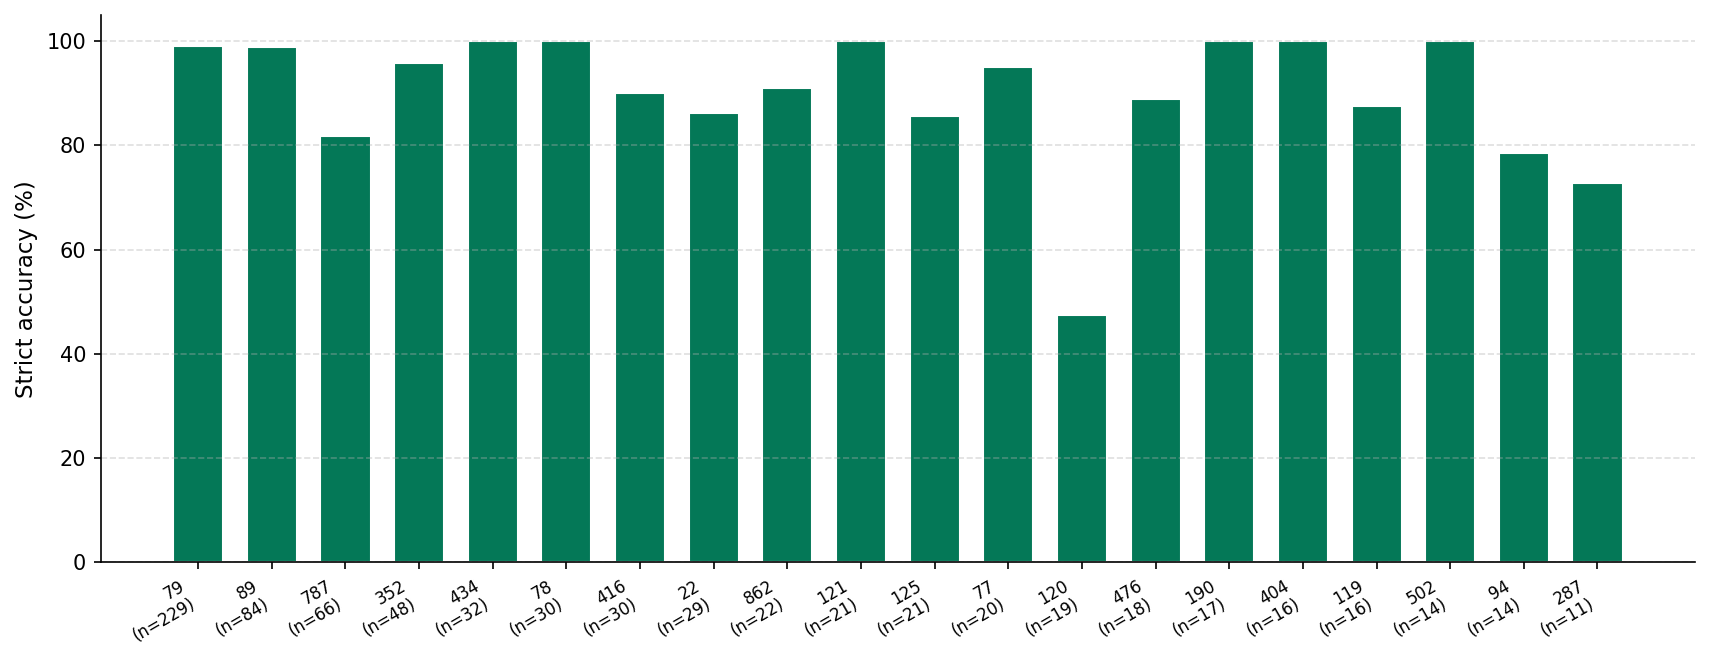
\includegraphics[width=0.95\textwidth]{figures/per_cwe_chart.png}
\caption{Per-CWE strict accuracy for the shipped Phi-4-mini-reasoning context-only clean-prompt RAG run on the 20 most-frequent CTI-Bench RCM CWEs ($n$ = sample count per CWE).}
\label{fig:per-cwe}
\end{figure*}

\subsection{Failure-Mode Typology}
\label{sec:failure-typology}

We classified mapped-subset failures from the four context-only clean-prompt RAG rows in Table~\ref{tab:model-mode-results}. The dominant category for Phi-4-mini-reasoning, Granite, and Gemma is cases where the system emits NVD's structured CWE but the CTI-Bench gold label is a different CWE---i.e., the system is faithful to NVD and the benchmark disagrees with NVD. DeepSeek is the exception: the clean prompt often causes it to produce long explanatory text without a terminal CWE identifier, which is consistent with the prompt-sensitivity pattern observed in Table~\ref{tab:model-mode-results}. Table~\ref{tab:mapped-failures} summarizes the mapped-failure distribution across models. Because NVD-unmapped CVEs have no structured CWE bridge, we classify their failures separately by whether the gold CWE survived context assembly and whether the model selected a retrieved or outside-context CWE; Table~\ref{tab:unmapped-failures} reports this distribution for the same clean-prompt runs.

\begin{table*}[!t]
\centering
\scriptsize
\renewcommand{\arraystretch}{1.15}
\setlength{\tabcolsep}{4pt}
\caption{Mapped-subset failure triage across all context-only clean-prompt RAG runs. Entries are count and percentage of that model's mapped failures; model headers show the total number of mapped failures out of 903 mapped queries.}
\label{tab:mapped-failures}
\begin{tabularx}{0.98\textwidth}{@{}Ycccc@{}}
\toprule
\textbf{Failure category} &
\textbf{DeepSeek-R1-8B} &
\textbf{Granite 4.1-8B} &
\textbf{Phi-4-mini} &
\textbf{Gemma 4 E4B} \\
\midrule
\textbf{Total Mapped Failures} & \textbf{128} & \textbf{105} & \textbf{66} & \textbf{84} \\
\midrule
NVD disagrees with CTI-Bench, model follows NVD
& 61 (47.7\%) & 87 (82.9\%) & 53 (80.3\%) & 77 (91.7\%) \\
\addlinespace
LLM ignored bridge-injected CWE
& 11 (8.6\%) & 7 (6.7\%) & 7 (10.6\%) & 3 (3.6\%) \\
\addlinespace
NVD disagrees and model also drifted
& 5 (3.9\%) & 4 (3.8\%) & 6 (9.1\%) & 3 (3.6\%) \\
\addlinespace
Multi-NVD CWE, model selected non-gold candidate
& 1 (0.8\%) & 6 (5.7\%) & 0 (0.0\%) & 1 (1.2\%) \\
\addlinespace
No CWE-ID parsed from answer
& 50 (39.1\%) & 1 (1.0\%) & 0 (0.0\%) & 0 (0.0\%) \\
\bottomrule
\end{tabularx}

\vspace{1.5em}

\caption{NVD-unmapped failure triage across all context-only clean-prompt RAG runs. Entries are count and percentage of that model's unmapped failures; model headers show the total number of unmapped failures out of 97 unmapped queries. Categories are mutually exclusive and are assigned from the parsed final answer and final assembled context.}
\label{tab:unmapped-failures}
\begin{tabularx}{0.98\textwidth}{@{}Ycccc@{}}
\toprule
\textbf{Failure category} &
\textbf{DeepSeek-R1-8B} &
\textbf{Granite 4.1-8B} &
\textbf{Phi-4-mini} &
\textbf{Gemma 4 E4B} \\
\midrule
\textbf{Total Unmapped Failures} & \textbf{51} & \textbf{39} & \textbf{25} & \textbf{13} \\
\midrule
No CWE-ID parsed from answer
& 26 (51.0\%) & 15 (38.5\%) & 0 (0.0\%) & 0 (0.0\%) \\
\addlinespace
Gold CWE absent from final context
& 8 (15.7\%) & 10 (25.6\%) & 12 (48.0\%) & 12 (92.3\%) \\
\addlinespace
Gold present; model selected another retrieved CWE
& 16 (31.4\%) & 10 (25.6\%) & 12 (48.0\%) & 0 (0.0\%) \\
\addlinespace
Gold present; model selected outside-context CWE
& 1 (2.0\%) & 4 (10.3\%) & 1 (4.0\%) & 1 (7.7\%) \\
\bottomrule
\end{tabularx}
\end{table*}

For the shipped Phi-4-mini-reasoning run, 25 unmapped failures remain. Taxonomic distance between predicted and gold CWE shows a similar pattern: predicted CWEs are usually children, parents, or siblings of the gold CWE within the CWE hierarchy, indicating that residual errors are fine-grained boundary decisions rather than broad mis-identification of the weakness family.

The dominant theme is consistent across both subsets: for the three clean-prompt runs without a large formatting-failure mode, most remaining mapped errors reflect annotation disagreement between NVD's structured field and CTI-Bench's curated label rather than model failures, while unmapped errors concentrate in either context-miss cases or fine-grained choices among retrieved CWE neighbors. These results suggest that further gains require either adjudicating NVD/CTI-Bench label disagreement on mapped CVEs or improving retrieval for the unmapped subset, rather than simply changing the final-answer model.

\subsection{Runtime and Latency}
\label{sec:latency}

Phi-4-mini-reasoning issues exactly one final-answer call for every CTI-Bench query, for a total of 1{,}000 generator calls across the full benchmark. The pipeline issues no additional generator calls. The retrieval-side cross-encoder reranking step scores at most a handful of CWE candidate chunks per query and adds milliseconds. The shipped 3.8B primary is also substantially faster per query than the 8B comparison row. All experiments run on a single NVIDIA RTX 4090 GPU (24~GB VRAM).

\section{Discussion and Limitations}

\subsection{Two Regimes: Retrieval-as-Lookup vs.\ Retrieval-plus-Reasoning}

The mapped and unmapped subsets exercise different parts of the architecture. On the 903 NVD-mapped CVEs, the bridge injects the structured NVD weakness field and strips competing CWE candidates, so the final model mostly has to read and emit the supplied identifier; this path reaches 837/903 (92.7\%). On the 97 NVD-unmapped CVEs, no structured NVD label is available, so the system relies on nearest mapped-CVE evidence, cross-encoder-ranked CWE candidates, and the primary model's taxonomy reasoning; this path reaches 72/97 (74.2\%). The headline 90.9\% is therefore a weighted average of a lookup-dominated mapped path and a harder retrieval-plus-reasoning unmapped path, rather than evidence that every retrieval component contributes equally on every query.

\subsection{Model-Independence: RAG Carries the Result}
\label{sec:model-independence}

A natural concern with the 90.9\% headline is that Phi-4-mini-reasoning is a reasoning-distilled model and may contribute capability beyond the retrieval pipeline itself. Section~\ref{sec:rag-contribution} reports the zero-shot versus with-RAG breakdown across four open-source compact primary models from distinct post-training regimes. We unpack the four anchor rows below.

\paragraph{Phi-4-mini-reasoning, shipped primary (+73.0\,pp from RAG)} A 3.8B-parameter open-source reasoning distillation by Microsoft. Zero-shot it scores 17.9\%, the weakest of the four lineup models and lower than every published baseline in Table~\ref{tab:leaderboard}; the lowest published comparator, LLaMA3-8B, still scores 44.7\%. The model has very little memorized CWE taxonomy, but with our retrieval pipeline it reaches 90.9\%, the largest RAG contribution we measure: an absolute lift of 730 newly correct queries on the 1{,}000-query split. A model with less than half the parameter count of every other open-source LLM baseline on the leaderboard reaches CTI-RCM state of the art when paired with our retrieval pipeline. This isolates the retrieval pipeline, rather than memorized cybersecurity knowledge in the LLM weights, as the dominant contributor.

\paragraph{IBM Granite 4.1-8B, model-independence evidence (+22.0\,pp from RAG)} Granite is a general-purpose RAG-tuned instruct model \cite{ibm-granite-2026} with no cybersecurity continued pre-training, no reasoning post-training, no task-specific fine-tuning on CTI-Bench or any CVE-to-CWE corpus, and no native chain-of-thought capability. It approximates the lower bound on what an off-the-shelf non-cybersecurity LLM can contribute to this task. Under our pipeline and the same clean prompt used by the shipped primary, Granite reaches 85.6\%, up from 63.6\% zero-shot. The +22.0\,pp lift is attributable purely to retrieval and bridge injection. Even this configuration exceeds the strongest published open-source fine-tuned cybersecurity classifier (RoBERTa-base CVE-to-CWE at 75.6\% \cite{mosievskiy-2026}) by 10.0\,pp and exceeds GPT-4's published no-retrieval baseline (72.0\% \cite{alam-2024}) by 13.6\,pp.

\paragraph{DeepSeek-R1-Distill-Llama-8B, 8B reasoning-distilled comparison (+56.4\,pp from RAG)} An 8B-parameter general-purpose reasoning distillation from DeepSeek-R1 into the Llama-3.1-8B base \cite{deepseek-r1-2025,llama31-2024}. Zero-shot it scores 25.7\%; under our retrieval pipeline and the same clean prompt it reaches 82.1\%, a +56.4\,pp lift. This row is useful precisely because it surfaces prompt sensitivity: the retrieval pipeline still buys more than fifty percentage points, but this 8B reasoning-distilled model is less robust to the benchmark-clean prompt than Phi.

\paragraph{Gemma 4 E4B with native thinking (+20.7\,pp from RAG)} Gemma 4 E4B is a Google instruct model with an opt-in thinking mode. Even with thinking enabled it scores only 69.6\% zero-shot; our pipeline lifts it to 90.3\%. This is the smallest RAG contribution in the lineup but still exceeds the fine-tuned open-source specialist by 14.7\,pp.

Across the four anchor rows the conclusion is identical: relative to Granite's no-reasoning, RAG-tuned-instruct row, the other LLM choices add between $-3.5$ and $+5.3$ percentage points under the same clean prompt, while retrieval contributes between $+20.7$ and $+73.0$ percentage points. The choice of LLM still matters, but the choice of retrieval pipeline (or its absence) shifts the result by tens to hundreds of cases. The dominant contributor to the headline is retrieval, not the model.

\subsection{Reasoning Distillation vs.\ Cybersecurity Continued Pre-training}
\label{sec:distill-vs-pretrain}

Phi-4-mini-reasoning is a 3.8B-parameter general-purpose reasoning distillation by Microsoft, with no cybersecurity continued pre-training. Published cybersecurity-continued-pretrained 8B models sit at 67.8\%--75.3\% on CTI-Bench RCM \emph{without} retrieval \cite{yu-2025,kassianik-2025,yang-2026}; under our retrieval pipeline our 3.8B Phi-4-mini-reasoning primary reaches 90.9\%. The implication is that a compact general-purpose reasoning distillation paired with strong retrieval is competitive with substantially larger cybersecurity-continued-pretrained models evaluated without retrieval. The retriever supplies structured NVD evidence and cross-encoder-ranked CWE candidates directly to the prompt, so the final-answer model needs reasoning over the supplied context more than encoded cybersecurity knowledge. We ship the no-cyber-pre-train configuration because it lets the paper claim a clean ``general compact LLM + RAG'' result with no upstream cybersecurity-domain post-training, and with less than half the parameter count of every other open-source LLM baseline on the leaderboard.

\subsection{Validity and Limitations}

The comparison to GPT-4 should be interpreted as a deployment comparison, not a raw model-capability comparison. GPT-4 in CTI-Bench had no retrieval over NVD or CWE, while our system has access to public data that analysts normally use. The mapped subset is therefore partly RAG-as-lookup, reaching 92.7\%; the unmapped subset is the stricter reasoning test, where the system reaches 74.2\%.

The single-primary architecture preserves the published CTI-Bench final-answer constraint (one final-answer LLM call per query) and uses no benchmark labels at inference. The corpus is intentionally restricted to CVE and CWE sources for CTI-RCM; broader CTI tasks may require adding ATT\&CK, CAPEC, and other threat-intelligence sources.

\subsection{Ethical Considerations}

This work uses only public NVD CVE records, public CWE definitions, and public benchmark prompts. It does not generate exploit code, disclose previously unknown vulnerabilities, or involve human subjects. Outputs should be treated as analyst decision-support recommendations rather than authoritative vulnerability assignments, since incorrect CWE mappings can misdirect remediation. The shipped configuration runs locally on consumer GPUs, so deployment does not require transmitting vulnerability records to third-party services.

\subsection{Non-Adopted Alternatives}
\label{sec:non-adopted}

The \emph{instruction prompt} is the experiment-only alternative to the shipped context-only prompt described in Section~\ref{sec:prompt}. It introduces task-specific instructions---an explicit CVE-to-CWE mapping framing, a directive to return the bridge-injected CWE when present, a no-refusal rule, and a one-line CWE-identifier output format (Appendix~\ref{app:prompt-instruction}). Table~\ref{tab:model-mode-results} reports both prompt variants for all four candidate primary models.

The cross-model split is informative. Phi-4-mini-reasoning (the shipped primary) and Gemma 4 E4B both score highest under the minimal context-only prompt, because their default chat templates already enforce concise output and additional instructions distract more than they constrain. DeepSeek-R1-Distill-Llama-8B and IBM Granite 4.1-8B instead prefer the directive instruction prompt. DeepSeek's reasoning distillation produces long chain-of-thought preambles unless explicit output-format constraints are present; under the context-only prompt the 8B DeepSeek variant frequently exhausts its token budget without emitting a terminal CWE identifier. Granite gains across both subsets when the prompt makes the CVE-to-CWE framing and the no-refusal directive explicit. Since the goal of this paper is to ship the highest benchmark-clean configuration rather than each model's per-row best prompt, we keep the context-only prompt as the reported final method and treat the instruction prompt purely as an experiment. The model-independence claim of Section~\ref{sec:rag-contribution} remains intact under this stricter comparison: every clean-prompt RAG row still lifts the corresponding zero-shot baseline by at least 20.7 percentage points.

\subsection{Future Work}
\label{sec:future-work}

Four directions address the remaining failure modes. (1)~Domain-adapted retrieval: a cross-encoder fine-tuning recipe with stronger false-negative filtering \cite{moreira-2024} may reduce context misses on the unmapped subset. (2)~Catastrophic-forgetting-aware fine-tuning: distillation-based RAG fine-tuning \cite{huang-2025} may improve near-miss failures without regressing easy cases. (3)~Stronger general-purpose reasoning distillations: as newer R1-style distillations become available, swapping in a stronger student should further raise unmapped accuracy without reintroducing domain post-training. (4)~Benchmark labeling: an inter-annotator-agreement audit of CTI-Bench's CWE labels would clarify how much of the residual error reflects model failure versus label noise; our triage suggests that label disagreement accounts for a large share of the remaining mapped failures.

\section{Conclusion}

This paper presented a Graph-Augmented Hybrid RAG system for CVE-to-CWE root-cause mapping. Using only public NVD and CWE data, and a single 3.8B general-purpose reasoning-distilled model (Phi-4-mini-reasoning) as the primary final-answer model, the system reaches 90.9\% strict accuracy on CTI-Bench RCM. This exceeds the published GPT-4 no-retrieval baseline by 18.9 percentage points and the strongest open-source published baseline by 15.3 percentage points, while the shipped primary uses less than half the parameter count of every other open-source LLM baseline on the leaderboard. The system runs locally on consumer hardware and uses no cybersecurity continued pre-training or task-specific fine-tuning of the final-answer model.

The main lesson is that careful retrieval design, paired with a compact off-the-shelf general-purpose local model, can match closed cybersecurity systems on a cybersecurity taxonomy task without cybersecurity-domain or task-specific post-training of the generator. Bridge injection resolves most NVD-mapped cases, while weighted k-NN voting and cross-encoder reranking improve the harder unmapped cases. Our four-model RAG-contribution analysis shows that retrieval contributes between +20.7 and +73.0 percentage points across distinct post-training regimes, while the choice of LLM only shifts the final score by a few cases on top of that. Beyond these gains, our failure analysis indicates that further improvement depends partly on adjudicating annotation disagreement between NVD and CTI-Bench and partly on improving retrieval for the unmapped subset.

\section*{LLM Usage Statement}

LLMs were used for editorial purposes in this manuscript, and all outputs were inspected by the authors to ensure accuracy and originality. The authors also used a general-purpose large language model for LaTeX formatting and bibliography organization. The manuscript was initially drafted by the authors.

\appendices

\section{Prompt Templates}
\label{app:prompts}

This appendix provides the verbatim prompt templates evaluated in our study.

\subsection{Context-Only Clean Prompt (Shipped Primary)}
\label{app:prompt-context-only}

The context-only clean prompt template is the benchmark-clean prompt used for the shipped primary model configuration (Phi-4-mini-reasoning). It contains only the retrieved evidence and the original CTI-Bench prompt question.

\begin{quote}\small\ttfamily
Retrieved evidence:\\
\{context\}\\
\\
\{question\}\\
\\
ANSWER:
\end{quote}

\subsection{Instruction Prompt (Experiment-Only)}
\label{app:prompt-instruction}

The alternative instruction prompt template includes explicit task-specific mapping instructions, a no-refusal directive, and output format constraints.

\begin{quote}\small\ttfamily
Map the CVE description to exactly one CWE ID.\\
\\
Use the provided context as evidence.\\
If the context contains an explicit CWE ID for this CVE, return that CWE ID.\\
If no explicit CWE ID is available, infer the best CWE from the CVE description and retrieved CWE definitions.\\
\\
Never refuse.\\
Never say there is not enough information.\\
Return one brief justification sentence.\\
The final line must contain only the CWE ID.\\
\\
Context:\\
\{context\}\\
\\
Question:\\
\{question\}\\
\\
Answer:
\end{quote}


\bibliographystyle{IEEEtran}
\bibliography{references}

\end{document}
